% XCircuit output "circ.tex" for LaTeX input from circ.ps
\def\putbox#1#2#3#4{\makebox[0in][l]{\makebox[#1][l]{}\raisebox{\baselineskip}[0in][0in]{\raisebox{#2}[0in][0in]{\scalebox{#3}{#4}}}}}
\def\rightbox#1{\makebox[0in][r]{#1}}
\def\centbox#1{\makebox[0in]{#1}}
\def\topbox#1{\raisebox{-0.60\baselineskip}[0in][0in]{#1}}
\def\midbox#1{\raisebox{-0.20\baselineskip}[0in][0in]{#1}}
   \scalebox{0.5826}{
   \normalsize
   \parbox{10.6979in}{
   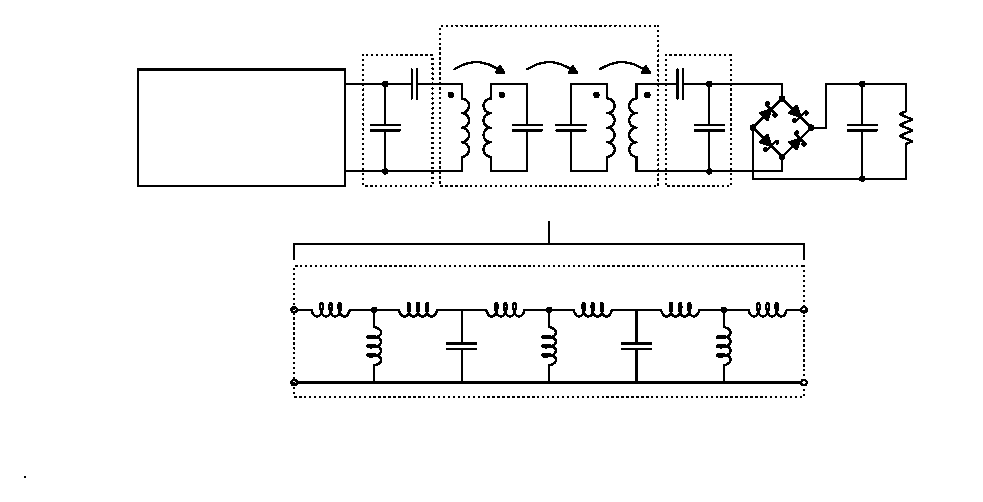
\includegraphics[scale=1.71644]{circ}\\
   % translate x=2193 y=969 scale 0.22
   \tiny
   \putbox{5.13in}{5.01in}{1.20}{k$_{12}$}%
   \putbox{5.93in}{5.01in}{1.20}{k$_{23}$}%
   \putbox{6.80in}{5.01in}{1.20}{k$_{34}$}%
   \putbox{2.09in}{4.34in}{1.20}{Class E }%
   \putbox{1.72in}{4.01in}{1.20}{Power Amplifer}%
   \putbox{1.43in}{3.68in}{1.20}{6.78 MHz RF Out}%
   \putbox{5.51in}{3.13in}{1.20}{Coil System}%
   \putbox{7.43in}{3.13in}{1.20}{Matching}%
   \putbox{3.93in}{3.13in}{1.20}{Matching}%
   \putbox{10.34in}{4.01in}{1.20}{Load}%
   \putbox{3.26in}{2.22in}{1.20}{(1-k$_{12}$)L}%
   \putbox{4.26in}{2.22in}{1.20}{(1-k$_{12}$)L}%
   \putbox{4.30in}{1.51in}{1.20}{k$_{12}$L}%
   \putbox{5.38in}{1.51in}{1.20}{C}%
   \putbox{5.26in}{2.22in}{1.20}{(1-k$_{23}$)L}%
   \putbox{6.26in}{2.22in}{1.20}{(1-k$_{23}$)L}%
   \putbox{7.26in}{2.22in}{1.20}{(1-k$_{34}$)L}%
   \putbox{8.26in}{2.22in}{1.20}{(1-k$_{34}$)L}%
   \putbox{7.38in}{1.51in}{1.20}{C}%
   \putbox{6.30in}{1.51in}{1.20}{k$_{23}$L}%
   \putbox{8.30in}{1.51in}{1.20}{k$_{34}$L}%
   \putbox{2.38in}{5.13in}{1.20}{Transmitter Side}%
   \putbox{8.09in}{5.09in}{1.20}{Receiver Side}%
   } % close 'parbox'
   } % close 'scalebox'
   \vspace{-\baselineskip} % this is not necessary, but looks better
